%%%
%%% Fortgeschrittenes Datenhandling
%%%
\part{Fortgeschrittenes Datenhandling}
\begin{frame}
\thispagestyle{empty}
\textbf{\huge{Fortgeschrittenes\\ Datenhandling}}
\end{frame}

\begin{frame}{Fortgeschrittenes Datenhandling Inhalt}
 \tableofcontents
\end{frame}

\section{by}
\begin{frame}[fragile]{by I} \index{by} \index{by!bysort}
Einzelne Ausprägungen ansprechen
\begin{lstlisting}
  summarize hhinc if edu == 1
  summarize hhinc if edu == 2
\end{lstlisting}
\hspace{1cm}\vdots
\begin{lstlisting}
  summarize hhinc if edu == 7
\end{lstlisting}

Alle gleichzeitig ansprechen
\begin{lstlisting}
  by edu, sort: summarize hhinc
\end{lstlisting}

  \begin{tikzpicture}[transform shape, rotate=10, overlay]
\node at (7.5,-0.5) [mybox] (box) {%
    \begin{minipage}[t!]{0.35\textwidth}
    \tiny\textcolor{black}{\texttt{by funktioniert nicht mit jedem Befehl, im Zweifel in die Hilfe gucken. Für by müssen die Fälle sortiert werden. Alternativ: bysort}}
    \end{minipage}
    };
\end{tikzpicture}
\end{frame}

\begin{frame}[fragile]{by II}
Es können auch mehrere Variablen genommen werden \index{by}
\begin{lstlisting}
  by sex edu, sort: summarize hhinc
\end{lstlisting}
\end{frame}

\section{in}
\begin{frame}[fragile]{in}
Wenn nur ausgewählte Fälle interessieren \index{list}
\begin{lstlisting}
  ** Nur die erste Beobachtung
  list sex in 1
  ** Beobachtungen 1 bis 10
  list sex in 1/10
\end{lstlisting}

  \begin{tikzpicture}[transform shape, rotate=10, overlay]
\node at (7.5,-0.5) [mybox] (box) {%
    \begin{minipage}[t!]{0.35\textwidth}
    \tiny\textcolor{black}{\texttt{Im Regelfall interessieren immer alle Fälle, wenn nicht, dann ist irgendetwas seltsames los.}}
    \end{minipage}
    };
\end{tikzpicture}
\end{frame}


\section{Schleifen}
\begin{frame}[fragile]{Schleifen I} \index{Schleifen} \index{Schleifen!foreach}
Schleifen in Stata. Beispiel aus \textcite[69f.]{Kohler2012}
\begin{lstlisting}
** Variablen r1 bis r10 erstellen
foreach var of newlist r1-r10 {
  gen `var' = runiform()
}

** Numerische Liste
foreach num of numlist 1/10 {
  replace r`num' = runiform()
}
\end{lstlisting}
\end{frame}

\begin{frame}[fragile]{Schleifen II} \index{Schleifen} \index{Schleifen!foreach} \index{Schleifen!forvalues}
\begin{lstlisting}
** Mehrere Ausdrücke in einer Schleifen
foreach var of varlist ybirth income {
  summarize `var', meanonly
  generate `var'_c = `var' - r(mean)
  label variable `var'_c "`var' (centered)"
}
\end{lstlisting}

\begin{lstlisting}
** Forvalues
forvalues num = 1/10 {
  replace r`num' = runiform()
}
\end{lstlisting}
\end{frame}

\section{log-Files}
\begin{frame}[fragile]{log-Files} \index{log} \index{log!log-Files}
  \begin{itemize}
    \item Auswertungen werden in log-Files gespeichert.
    \item In die log-Files werden die Befehle und der Output geschrieben.
    \item Das loggen erfolgt nach 
    \begin{lstlisting}
  log using <dateiname.log>
    \end{lstlisting}
    \item Stata Logfiles können mit jedem Texteditor geöffnet werden.
  \end{itemize}
\end{frame}

\begin{frame}[fragile]{LogfilesII}
  \begin{itemize} \index{log} \index{log!using} \index{log!close}
   \item log-File einstellen. Dieses sollte aus Gründen der Übersicht heißen, wie das do-File, welches das log-File erstellt. 
   \begin{lstlisting}
  log using read-soep.log, replace
   \end{lstlisting}
   \item Am Dateiende das Log-File schließen.
   \begin{lstlisting}
  ** Befehle nach log close werden nicht mehr geloggt
  log close
   \end{lstlisting}
     \item Bei Fehlern im do-File kann es nötig sein, dass log-File manuell zu schließen
     \begin{lstlisting}
  log close
     \end{lstlisting}
  \end{itemize}
\end{frame}

\section{Macros}
\begin{frame}[fragile]{Macros} \index{Macros} \index{Macros!global}
Hin und wieder empfiehlt es sich, sogenannte Macros zu verwenden. Ein solches Macro kann z.~B. global definiert werden.
\begin{lstlisting}
  ** global Macroname Pfadname
  global DATA "D:/Daten/data/original/"
  global OUT "D:/Daten/data/bearbeitet/"
\end{lstlisting}
Die Macros enthalten jetzt die Pfadangabe
\begin{lstlisting}
 cd "${DATA}"
\end{lstlisting}

\end{frame}

\begin{frame}[fragile]{Macros II}
Diese können nun aus dem do-File aufgerufen werden. \index{Macros}
\begin{lstlisting}
  use "${DATA}testdaten.dta", clear
  save "${OUT}testdaten_rekodiert.dta", replace
\end{lstlisting}
Dadurch wird die Syntax wieder lesbarer.

  \begin{tikzpicture}[transform shape, rotate=10, overlay]
\node at (7.5,-2.1) [mybox] (box) {%
    \begin{minipage}[t!]{0.35\textwidth}
    \tiny\textcolor{black}{\texttt{Sie sparen sich Tippzeit. Lange Pfade müssen nur einmalig eingegeben werden, dadurch sinkt die Fehleranfälligkeit. Ein Macro was einmal richtig ist, ist das ganze Dokument über richtig. Macros übernehmen aber nicht das Denken.}}
    \end{minipage}
    };
\end{tikzpicture}

\end{frame}

\section{Using}
\begin{frame}[fragile]{using} \index{Laden!use using} \index{Sortieren!sort}
Stata kann nur eine begrenzte Anzahl Variablen handeln, daher sollte man diese ein wenig im Blick behalten.\footnote{Je nach Version hat Stata ein unterschiedliches Limit an Variablen: IC (die Version aus dem CIP-Raum) $2,047$, ab SE $32,767$. Mehr Variablen lässt sich Stata aber auch gut bezahlen. Preise 2013: \$189 und \$395 für Studenten. Nicht akademische Einzelplatzlizenzen \$$1545$ und \$$2090$.} Deshalb nicht immer alle Variablen einlesen
\begin{lstlisting}
  ** Sehr schmalen ppfad einlesen
  ** behält nur hhnr persnr sex gebjahr
  use hhnr persnr sex gebjahr using "${DATA}ppfad.dta"
  ** Anschließend Fälle sortieren
  sort persnr gebjahr
\end{lstlisting}
\end{frame}

\section{Merge}
\begin{frame}{merge} \index{Merge!merge}
\begin{minipage}{11cm}
Im hier verwendeten Datensatz, dem Sozio-oekonomischen Panel (SOEP) (s. \cite{Wagner07}), sind die Datensätze eines jeden Jahres in verschiedene Datenfiles aufgeteilt. Das hat zum Teil historische, möglicherweise auch praktische Gründe.\\
Ausgehend von einem gemeinsamen Datenfile, können die anderen Datenfiles hinzugespielt werden. Dieses hinzuspielen wird \textit{mergen} genannt.
\end{minipage}
\end{frame}

\begin{frame}[fragile]{merge II} \index{Merge!merge}
\begin{minipage}{11cm}
Wir müssen also unter Umständen aus anderen Datenfiles zum Beispiel aus \textbf{bckind} und \textbf{bcpgen} Informationen an unseren Datensatz ppfad anspielen. Damit den richtigen Personen die richtigen Informationen zugespielt werden, werden die Haushaltsnummer (hhnr) und die Personennummer (persnr) als Referenz genommen.\\

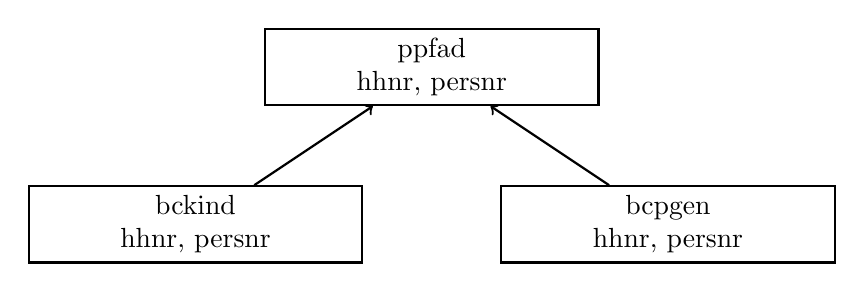
\begin{tikzpicture}[thick]
\node at ( 3,2) [rectangle,draw=black,text width=4cm,align=center] (ppfad) {ppfad \\
									    hhnr, persnr};

\node at ( 0,0) [rectangle,draw=black,text width=4cm,align=center] (bckind) {bckind \\
									    hhnr, persnr};
\node at ( 6,0) [rectangle,draw=black,text width=4cm,align=center] (bcpgen) {bcpgen \\
									    hhnr, persnr};
									    
\draw[->] (bckind) -- (ppfad);
\draw[->] (bcpgen) -- (ppfad);
\end{tikzpicture}
\end{minipage}
\end{frame}


\begin{frame}[fragile]{merge III}
Der \texttt{merge}-Befehl wird aufgerufen. \index{Merge!merge}

\begin{lstlisting}
  ** merge ppfad mit 2011 bbp
  merge 1:1 persnr using "${DATA}bbp.dta"
\end{lstlisting}

\begin{table}
\begin{center}
\begin{scriptsize}
\begin{tabular}{lll}
 Result & \# of obs. & \\ 
 \midrule
 not matched & 25,834 & \\
 ~~from master & 25,834  &(\_merge==1) \\
 ~~from using  & 0 &(\_merge==2) \\
 & & \\
 matched & 10,471 & (\_merge==3) \\
 \midrule
\end{tabular}
\end{scriptsize}
\end{center}
\end{table}

\end{frame}

\begin{frame}[fragile]{merge IV}\index{Merge!\_merge}\index{Merge!merge}
\begin{minipage}{11cm}
Es gibt nun verschiedene Möglichkeiten. Im Folgenden werden alle \texttt{\_merge==2} Fälle gelöscht. Beobachtungen also, die nicht in \textbf{ppfad} vorkommen, wohl aber im hinzugespielten Datenfile. \texttt{\_merge==1} würde die Fälle löschen, bei denen ein Eintrag aus \textbf{ppfad} nicht im hinzugespielten Datenfile ist, \texttt{\_merge==3}, wenn Beobachtungen übereinstimmen.
\begin{lstlisting}
  ** Drop wenn using nicht in master ist
  drop if _merge==2
  ** _merge droppen
  drop _merge
\end{lstlisting}
\end{minipage}


  \begin{tikzpicture}[transform shape, rotate=10, overlay]
\node at (7.5,-1.5) [mybox] (box) {%
    \begin{minipage}[t!]{0.35\textwidth}
    \tiny\textcolor{black}{\texttt{Wann welcher merge gewählt wird, hängt nicht unerheblich von der dahinterliegenden Fragestellung ab.}}
    \end{minipage}
    };
\end{tikzpicture}

\end{frame}

\begin{frame}[fragile]{merge V} \index{Merge!merge} \index{Merge!merge, keepusing}
Beispiel: merge mit der generierten Variable des höchsten Bildungsabschlusses aus \textbf{bbpgen}.

\begin{lstlisting}
  merge 1:1 hhnr persnr using "${DATA}bbpgen.dta", keepusing(bbpsbil)
  drop if _merge==2
  drop _merge
\end{lstlisting}

  \begin{tikzpicture}[transform shape, rotate=10, overlay]
\node at (7.5,-1.5) [mybox] (box) {%
    \begin{minipage}[t!]{0.35\textwidth}
    \tiny\textcolor{black}{\texttt{In \textbf{bbpgen} sind $59$ Variablen, wir brauchen aber nur den Schulabschluss.}}
    \end{minipage}
    };
\end{tikzpicture}
\end{frame}

\section{Operatoren}
\begin{frame}[fragile]{Operatoren} \index{Operatoren}
Stata listet folgende Operatoren, die im Regelfall auch mit Variablen funktionieren. Bei \texttt{var1\^{}2} wird jede Beobachtung hoch zwei genommen.
\begin{lstlisting}
 == // gleich
 != // ungleich alternativ ~=
 & // und
 | // oder
 ! // nicht
 < // kleiner
 > // größer
 <= // kleiner gleich
 >= // größer gleich
 + // plus
 - // minus
 / // geteilt
 * // mal
 ^ // hoch
\end{lstlisting}
\end{frame}

\begin{frame}[fragile]{Funktionen} \index{Funktionen}
Darüberhinaus verfügt Stata über eine Reihe von eingebauten Funktionen (\texttt{help functions}).
Eine Auswahl:
\begin{lstlisting}
  abs() // Absolutwert/Betrag |-2| == 2
  max() // Größter Wert
  min() // Kleinster Wert
  exp() // e-Funktion
  ln() // Logarithmus
  round() // Runden
  sin() // Sinus
  sqrt() // Wurzel
  runiform() // Zufallszahlen
\end{lstlisting}
\end{frame}